% !TeX spellcheck = en_US

\documentclass{Bredelebeamer}




%%%%%%%%%%%%%%%%%%%%%%%%%%%%%%%%%%%%%%%%%%%%%%%%


\vspace{4cm}

\title{SAA - návrh projektu}

\subtitle{}

\author{Juraj Hledík}

\institute[]{NBS}

\date{2. februára 2022}
% Optionnel. La date, généralement celle du jour de la conférence

\subject{Title}
% C'est utilisé dans les métadonnes du PDF



%\titlegraphic{\vspace{1cm}\hspace*{6.75cm}~%
%   
\includegraphics[width=0.01\textwidth,natwidth=2cm,natheight=0.5cm]{images/VgsfLogo.eps}
%}

%
%\logo{
%
\includegraphics[scale=0.15]{images/logo.png}
%}
\usepackage{psfrag}
\usepackage{multirow}
\usepackage{tikz}
\usepackage{graphicx}
\usepackage{caption}
\usepackage{subfig}
\usepackage{amsmath}
\usetikzlibrary{arrows,shapes,trees}
\usepackage{color}

\usepackage{auto-pst-pdf} 
\usepackage{psfrag}
\usetikzlibrary{bayesnet}

\usepackage{appendixnumberbeamer}

%%%%%%%%%%%%%%%%%%%%%%%%%%%%%%%%%%%%%%%%%%%%%%%%%%%%%%%%%%%%%%%%%%%%%
\begin{document}

\begin{frame}
\titlepage
\end{frame}

%\begin{frame}
%	\frametitle{Budúcnosť IFP}
%	\vfill
%	\begin{itemize}
%		\item Budovanie reputácie cez:
%		\begin{itemize}
%			\item akademickú a odbornú excelentnosť produkovaných analýz,
%			\item aktívny vzťah s verejnosťou,
%			\item spoluprácu s inštitúciami (univerzity, NBS, RRZ).						
%		\end{itemize}
%	\end{itemize}
%\end{frame}

\begin{frame}{Témy}
\begin{block}{Cieľ, aktuálny stav}
	\begin{itemize}
	\item Strategická alokácia aktív
	\item Preferencie a obmedzenia
	\item Projekt doteraz	
	\end{itemize}
\end{block}


\pause\begin{block}{Predstava do budúcna}
	\begin{itemize}
		\item Odhad viacrozmerného rozdelenia výnosov pomocou vine kopúl
		\item Prametrizovateľná optimalizácia portfólia
		\item Výstup pre konečného používateľa
	\end{itemize}
\end{block}
\end{frame}

\section{Cieľ, aktuálny stav}
\subsection{Cieľ}

\begin{frame}{Cieľ, preferencie, obmedzenia}
	\begin{itemize}
		\item Skonsolidovať jednotlivé portfóliá / pozície NBS do jedného frameworku.
		\item Lepší prehľad o očakávanom výnose, koreláciach a vzájomných rizikách jednotlivých pozícií.
		\item Preferencie investora: optimalizácia vzhľadom na expected shortfall na rôznych hladinách a maturitách.
		\item Obmedzenia / reštrikcie:
		\begin{itemize}
			\item zafixované množstvo zlata
			\item zafixované intervenčné portfólio
			\item dynamicky sa meniace ASW portfólio (asset swap spreads)
			\item reputačné otázky pri strate resp. strate dva roky po sebe
			\item nekombinovať s MPO
		\end{itemize}
	\end{itemize}
\end{frame}

\subsection{Aktuálny stav}

\begin{frame}{Aktuálny stav projektu}
	\begin{itemize}
		\item Vybraných 8 reprezentatívnych indexov
		\begin{itemize}
			\item \textbf{Zlato} Gold XAU/EUR Rate FX Unhdg.
			\item \textbf{US Treasuries }1-5 Year US Govt (ICE) FX Unhdg.
			\item\textbf{ASW} 1-5 Year Global Non-Sov (ICE) IR hdg. IRS
			\item \textbf{Akcie } World Equity (MSCI) FX Unhdg.
			\item \textbf{Čínske vládne dlhopisy}  1-3 Year China Govt (ICE) FX Unhdg.
			\item \textbf{TIPS, infl. dlhopisy } US Inflation-Linked Govt (ICE) FX Hdg.
			\item \textbf{Mortgage - backed securities} US MBS (ICE) FX Hdg.
			\item \textbf{Emerging market, dlhopisy} EM global IG Govt (JPM) FX Hdg.
		\end{itemize}
		\pause\item Testy:
		\begin{itemize}
			\item Historické výnosy nie sú normálne rozdelené.
			\item Ne-normalita nie je spôsobená asymetriou, ale špicatosťou (kurtosis).
		\end{itemize}
		\pause\item Optimalizácia portfólia:
		\begin{itemize}
			\item Mean-Variance optimalizácia, Markowitz, predpokladaná normalita výnosov.
			\item Ex post výpočet pre expected shortfall.
			\item Zahrnutá nenormalita výnosov pomocou bootstrappingu.
			\item Vyčíslenie expected shortfall pre dané mean-variance optimálne portfólio.
		\end{itemize}
	\end{itemize}
\end{frame}

\section{Plán projektu}
\subsection{Plán projektu}

\begin{frame}{Čo vieme zlepšiť?}
	\begin{block}{Odhad budúcich výnosov}
		\begin{itemize}
			\item Finančné výnosy sú málokedy normálne rozdelené.
			\item Keďže investor má preferencie ohľadom expected shortfall, je kľúčové čo najpresnejšie modelovať "dolný chvost" výnosov.
			\item Ponúknuť alternatívu k bootstrappingu.
		\end{itemize}
	\end{block}
	
	\pause\begin{block}{Optimalizácia portfólia}
		\begin{itemize}
			\item Pri dobre odhadnutej distribúcii budúcich výnosov dáva zmysel porovnať rôzne investičné ciele a kritéria.
			\item Optimalizácia expected shortfallu je linearizovateľný problém.
		\end{itemize}
	\end{block}
	
	\pause\begin{block}{Sumarizácia medzi modelmi a preferenciami}
		\begin{itemize}
			\item Prehľadné dynamické zobrazenie výstupu, možnosť porovnania prístupov.
			\item Vzájomné porovnanie takto optimálnych portfólií je dobrým mechanizmom aj na feedback od investora ohľadom výberu konkrétneho spôsobu optimalizácie portfólia.
		\end{itemize}
	\end{block}

\end{frame}

\section{Kopuly}
\subsection{Kopuly}

\begin{frame}{Ako vyriešiť nenormalitu výnosov}
	\begin{itemize}
		\item Najčastejšie sa používajú metódy založené na kopulách.
		\item Kopula = modelovanie závislosti medzi viacerými náhodnými premennými.
		\item Pre náhodné premenné $X_1, \ldots, X_n$ s distribučnými funkciami $F(x_1), \ldots, F(x_n)$ majme vektor:\\
		\begin{equation}
			{\displaystyle (U_{1},U_{2},\dots ,U_{n})=\left(F_{1}(X_{1}),F_{2}(X_{2}),\dots ,F_{n}(X_{n})\right)}
		\end{equation}
		Z definície distribučnej funkcie má každá zložka tohto vektora rovnomerné rozdelenie na intervale $[0,1]$.
		\item Kopulou nad premennými $X_1, \ldots, X_n$ rozumieme distribučnú funkciu vektora $(U_{1},U_{2},\dots ,U_{n})$:
		\begin{equation}
			{\displaystyle C(u_{1},u_{2},\dots ,u_{n})=\Pr[U_{1}\leq u_{1},U_{2}\leq u_{2},\dots ,U_{n}\leq u_{n}].}		
		\end{equation}
		\item Celá informácia o rozdelení $X_1, \ldots, X_n$ je teda daná:
		\begin{itemize}
			\item Marginálnymi rozdeleniami $F(X_1), \ldots, F(X_n)$.
			\item Kopulou $C(u_{1},u_{2},\dots ,u_{n})$.
		\end{itemize}
		\item Sklarova veta: Pre viacrozmerné rozdelenie s hustotou $h(.)$, marginálnymi rozdeleniami $f_i(.)$ a kopulou $c(.)$ platí:
		\begin{equation}
			{\displaystyle h(x_{1},\dots ,x_{n})=c(F_{1}(x_{1}),\dots ,F_{n}(x_{n}))\cdot f_{1}(x_{1})\cdot \dots \cdot f_{n}(x_{n}),}
		\end{equation}
	\end{itemize}
\end{frame}

\begin{frame}{Bežné kopuly}
	\centering
	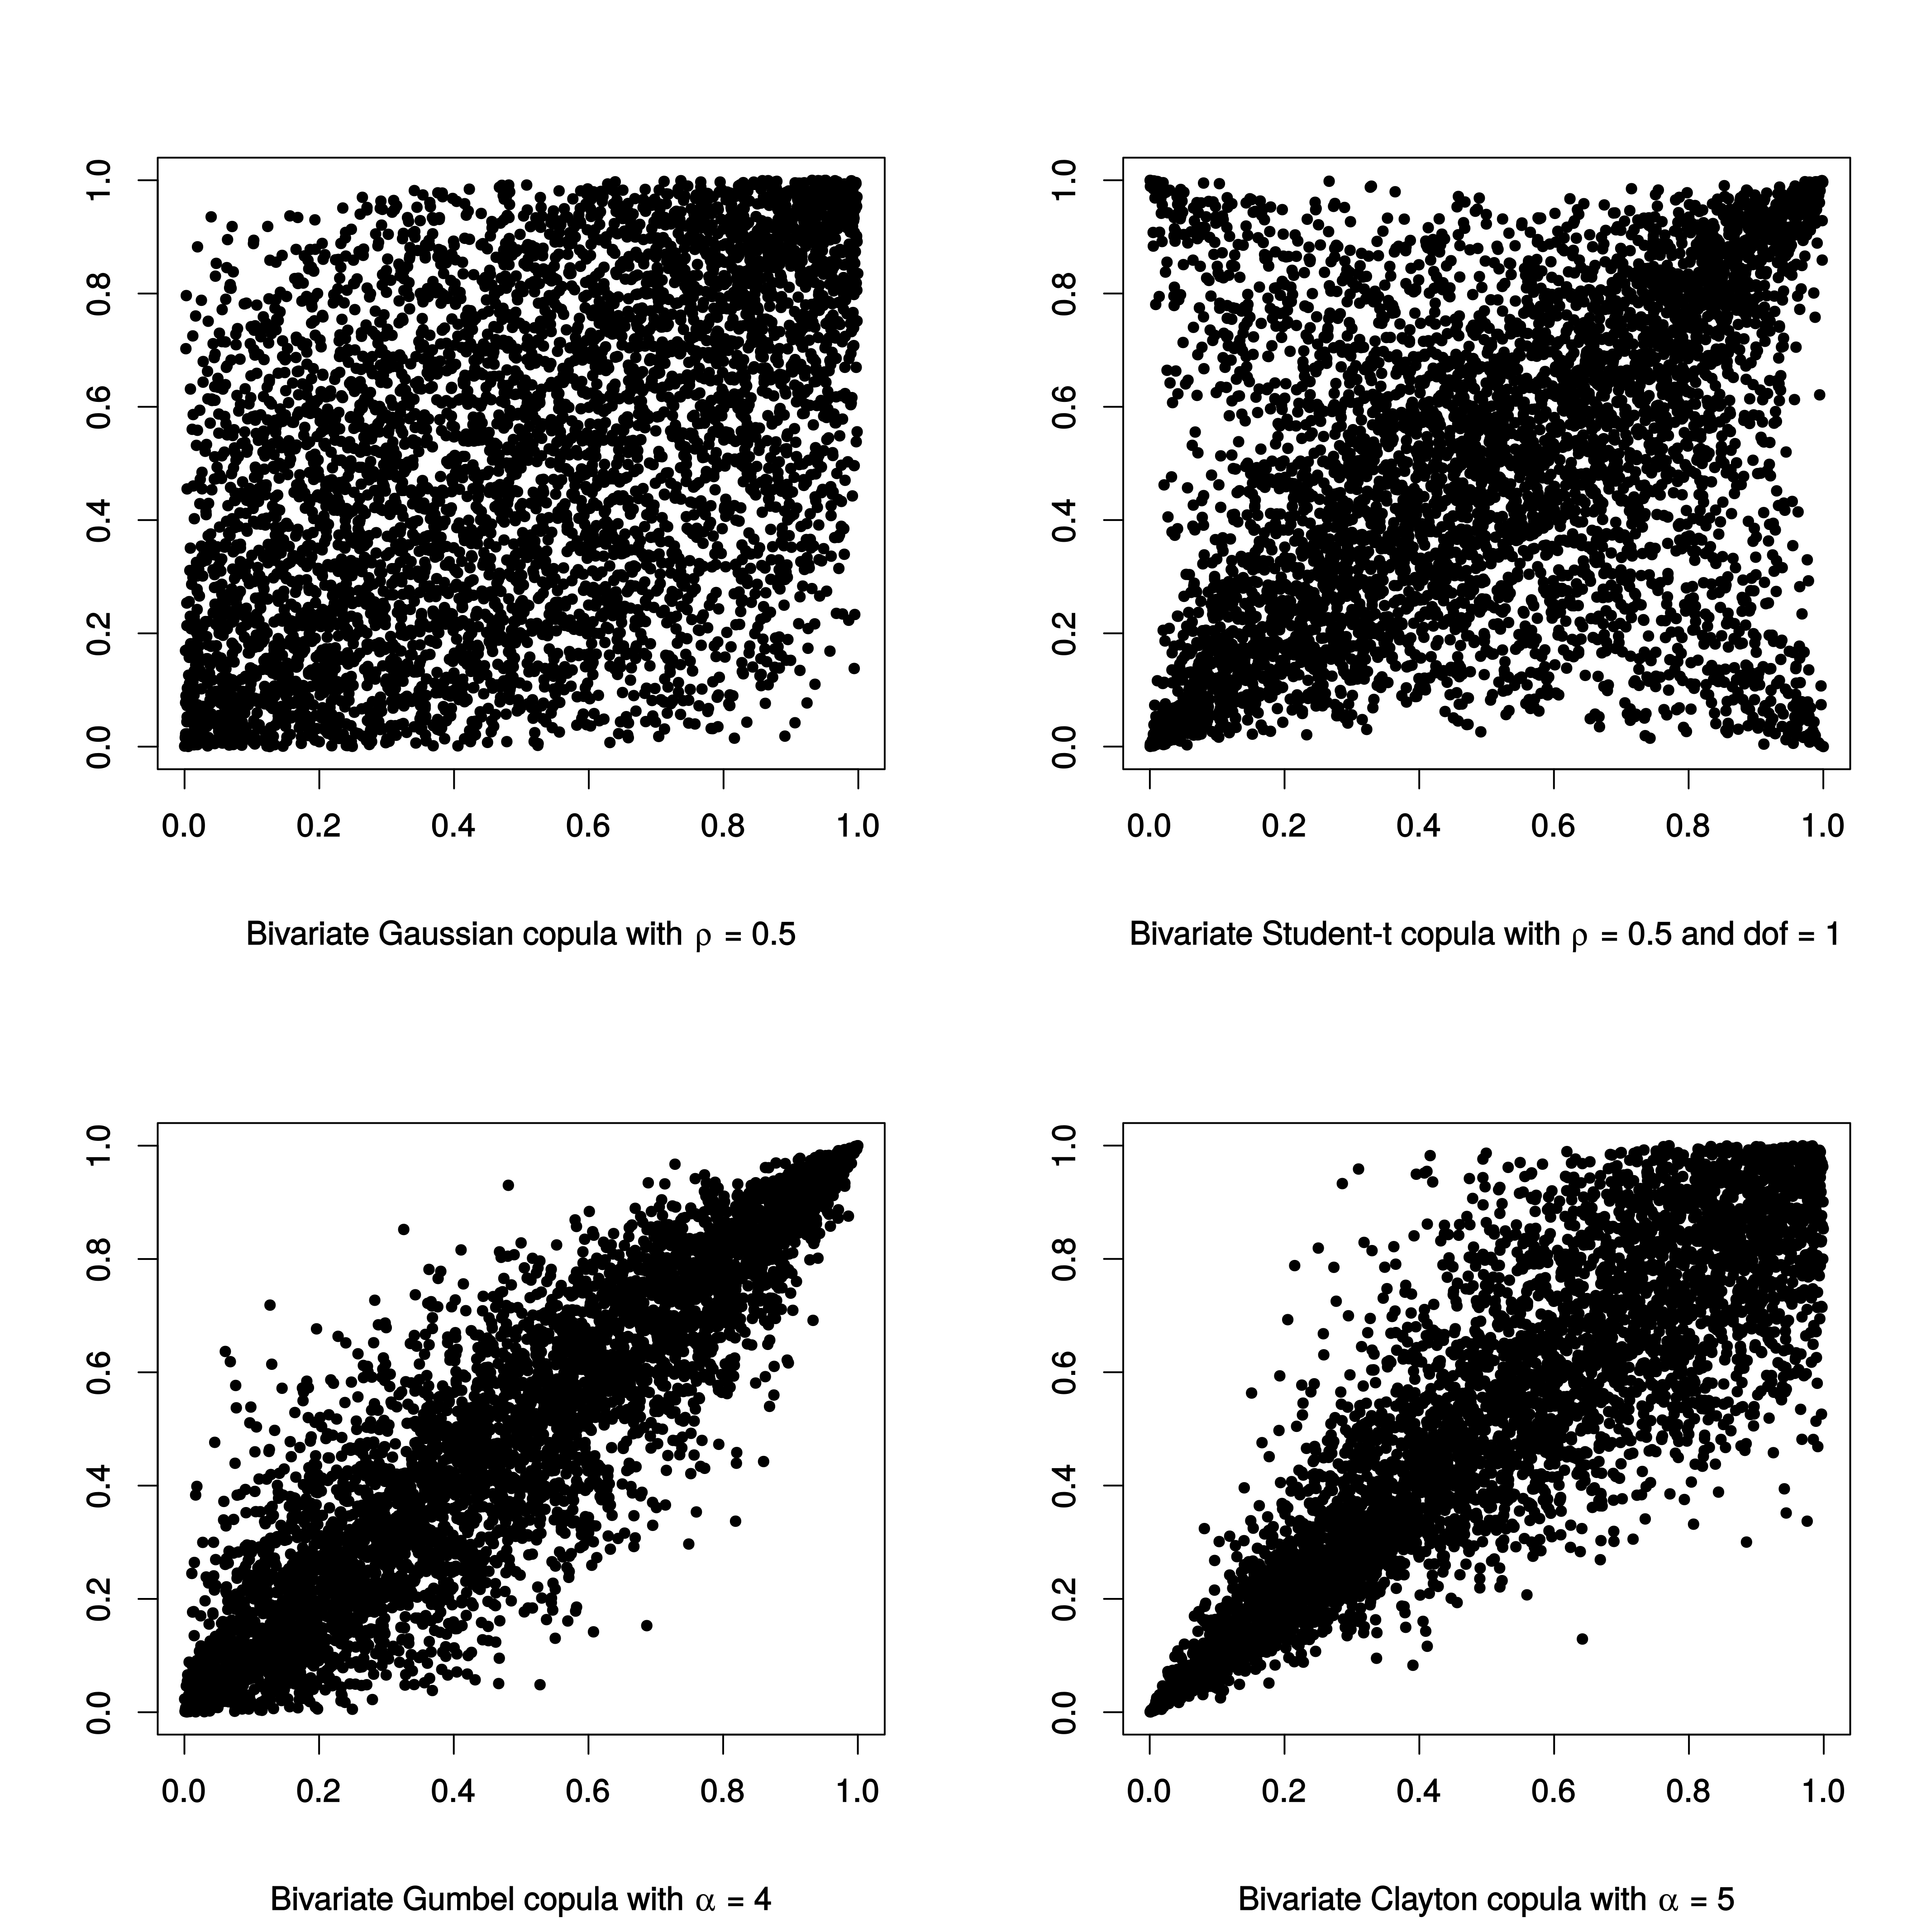
\includegraphics[width=0.71\textwidth]{Figures/Four_Correlations}
\end{frame}

\begin{frame}{Vine Copula}
	\begin{itemize}
		\item Problém pri vyšších dimenziách - len jeden / dva parametre.
		\item Možné riešenie - Vine Kopuly.
		\item Miesto jednej kopuly pre celé viacrozmerné rozdelenie použijeme kombináciu dvojrozmerných kopúl a správne definovaných podmienených rozdelení.
		\item Napríklad v troch rozmeroch vieme podmienenú hustotu $x_1$ vyjadriť ako:
		\begin{equation}
			f(x_1|x_2, x_3) = c_{12|3}(F_{1|3}(x_1|x_3), F_{2|3}(x_2|x_3))\cdot f(x_1|x_3).
		\end{equation}
		\item Alebo ekvivalentne aj takto:
		\begin{equation}
			f(x_1|x_2, x_3) = c_{13|2}(F_{1|2}(x_1|x_2), F_{3|2}(x_3|x_2))\cdot f(x_1|x_2).
		\end{equation}
		\item Ak zapíšeme pomocou kopuly aj $f(x_1|x_2)$, dostávame:
		\begin{equation}
			f(x_1|x_2, x_3) = c_{13|2}(F_{1|2}(x_1|x_2), F_{3|2}(x_3|x_2))\cdot c_{12}(F_1(x_1), F_2(x_2))\cdot f_1(x_1).
		\end{equation}
		\item Pri ďalších rozmeroch funguje postup analogicky - iteratívne.
	\end{itemize}
\end{frame}

\begin{frame}{D-vine kopula}
	\centering
	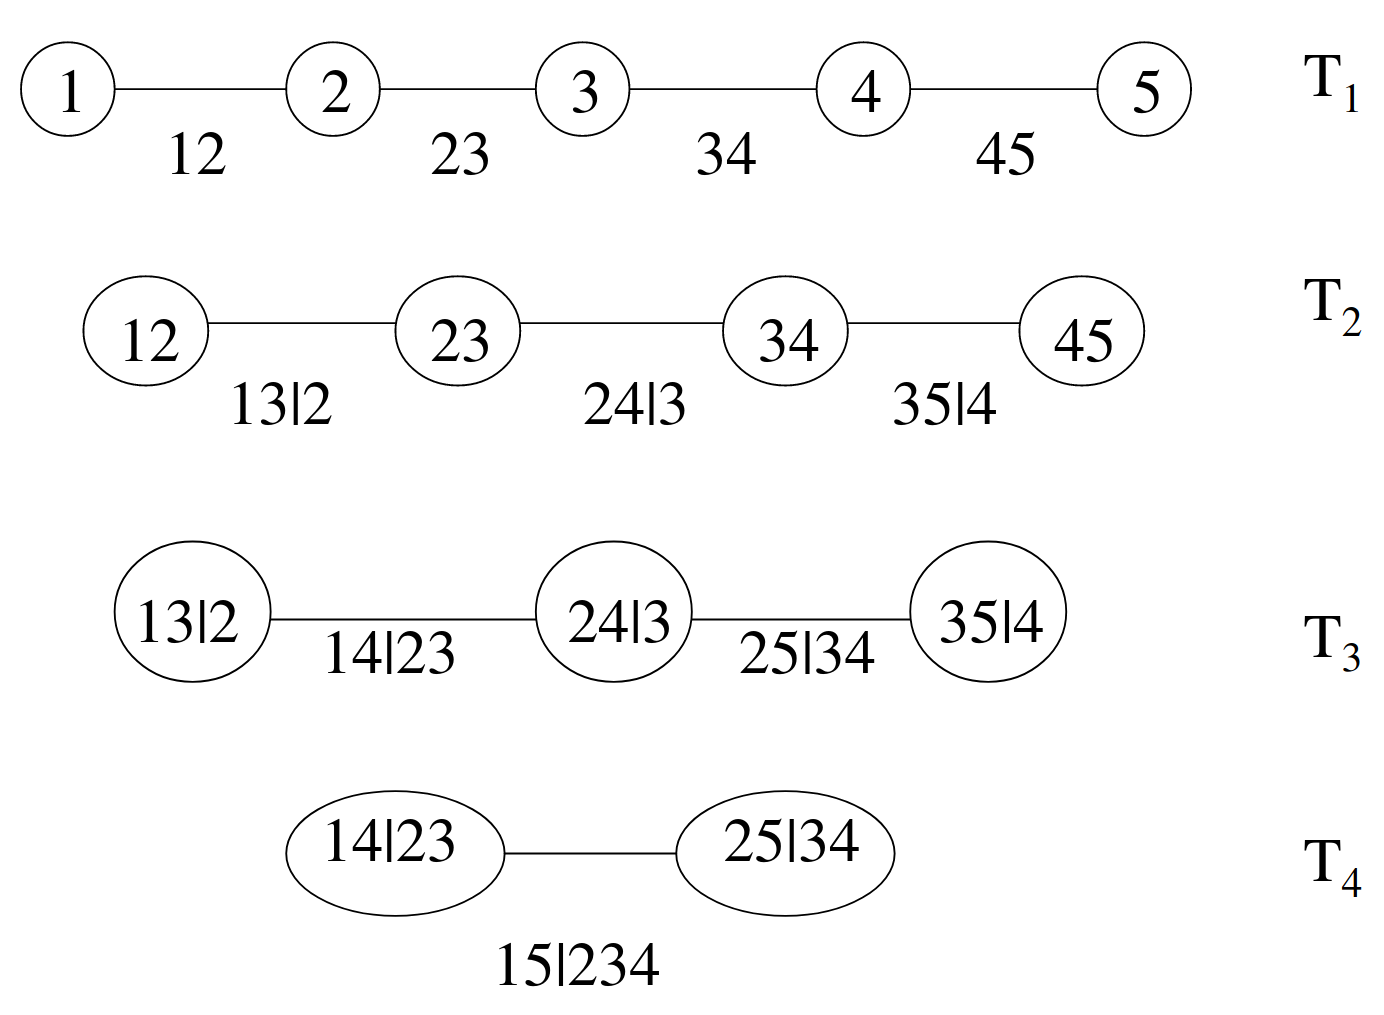
\includegraphics[width=0.9\textwidth]{Figures/d-vine}
\end{frame}

\begin{frame}{C-vine kopula}
	\centering
	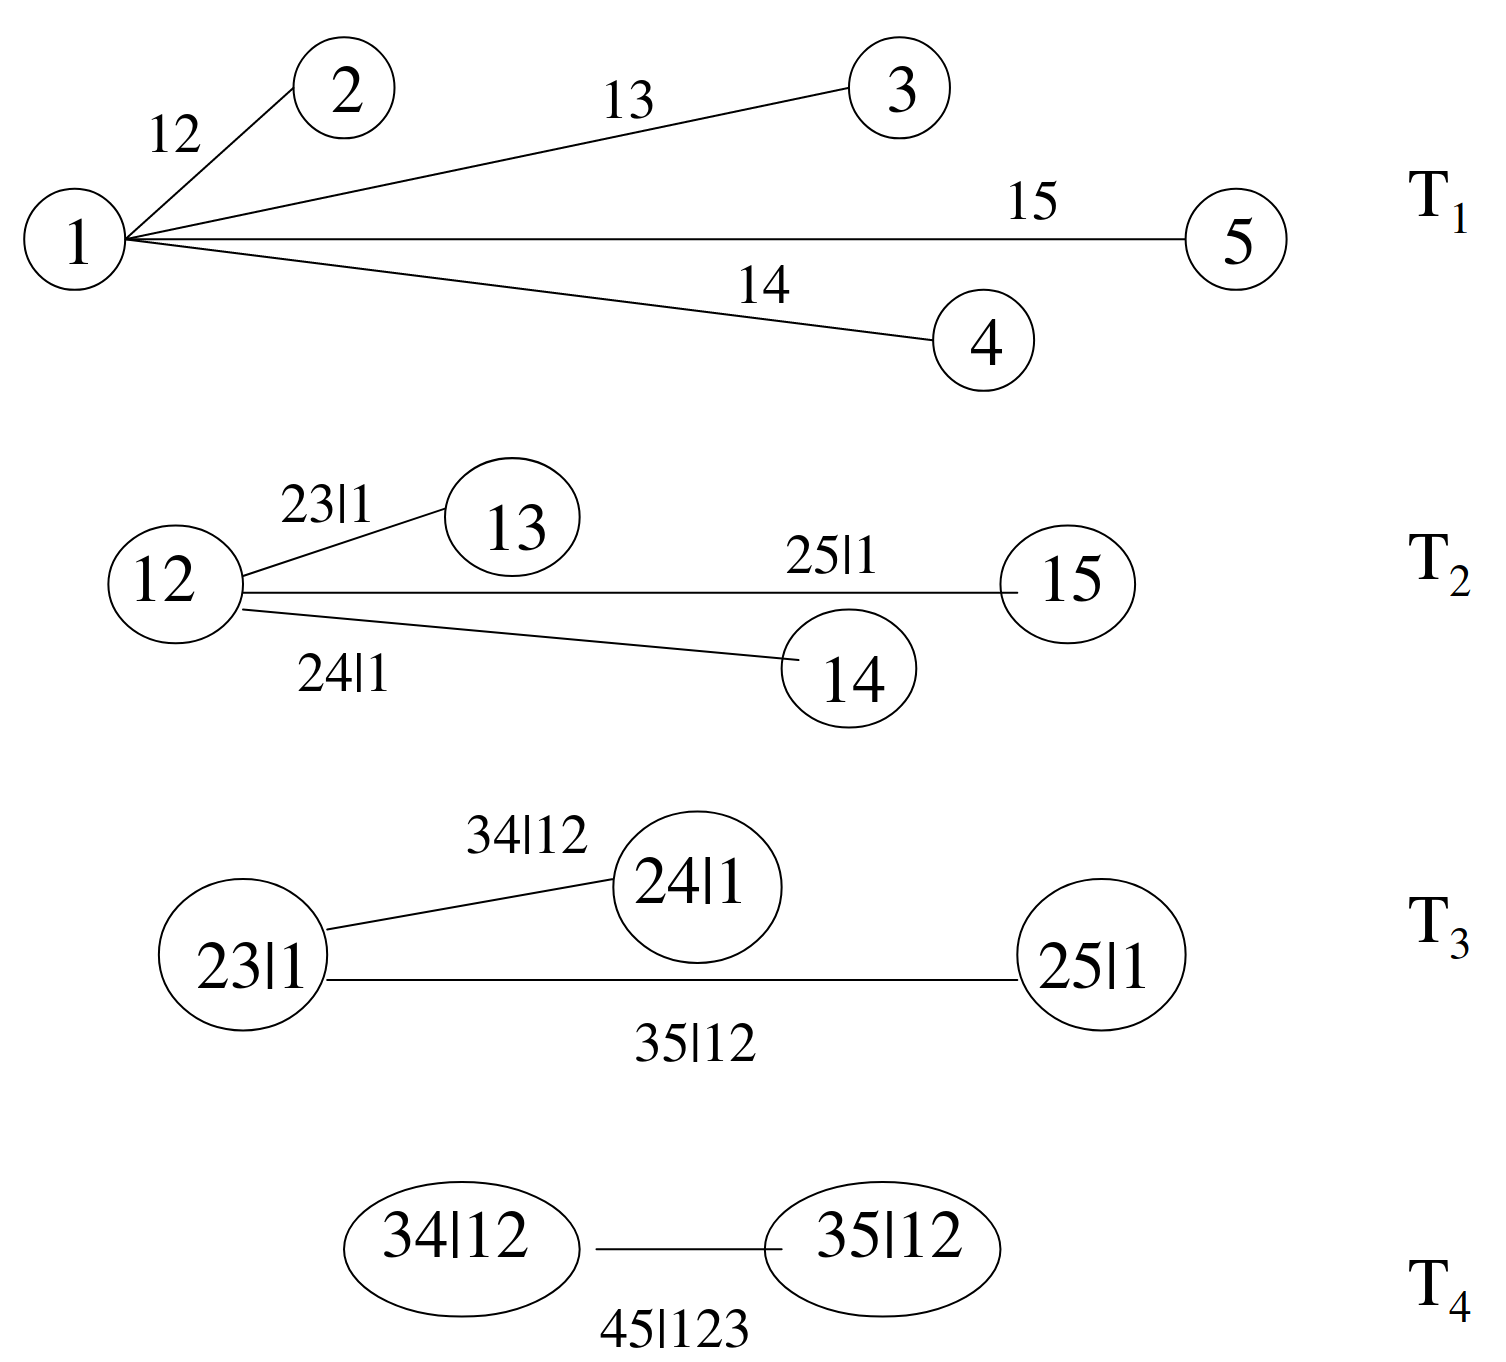
\includegraphics[width=0.7\textwidth]{Figures/c-vine}
\end{frame}

\begin{frame}{R-vine kopula}
	\centering
	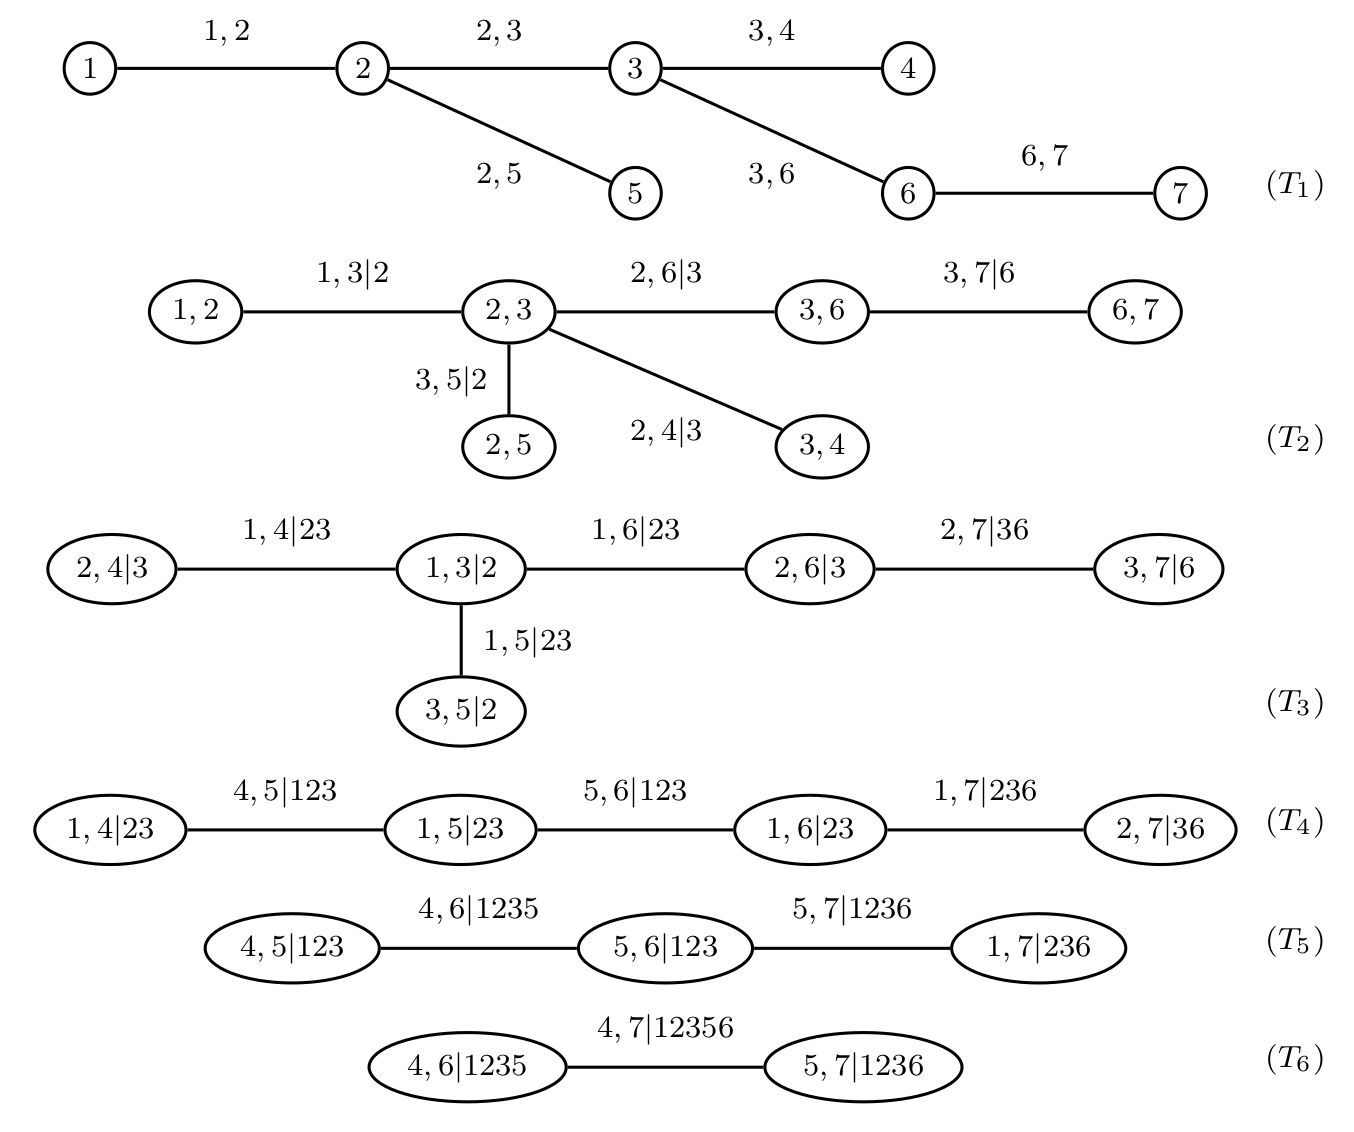
\includegraphics[width=0.8\textwidth]{Figures/r-vine}
\end{frame}

\section{Optimalizácia}

\begin{frame}{2 prístupy k SAA}
	\begin{itemize}
		\item Za\textbf{ fixné zložky} portfólia označme čokoľvek, čo nechceme nakupovať ani predávať - napr. zlato. V tomto zmysle slova je pre nás fixnou zložkou aj ASW portfólio, keďže jeho veľkosť nevieme dobre predpovedať ani nastaviť na základe výstupu nášho modelu. Berieme ho teda ako určitú formu ohraničenia optimalizácie.
		\pause\item Za \textbf{variabilné zložky} považujeme čokoľvek, čo vieme nakúpiť alebo predať na základe výstupu z modelu.
		\pause\item Pri optimalizácii portfólia by som chcel analyzovať dva rôzne praktické prístupy.
		\item \textbf{Scenár č.1 (viac menej stabilne veľké portfólio)} - Investor určí objem investície, ktorú chce vložiť do variabilných zložiek (napr. akcií). Model vyráta optimálne váhy vzhľadom na ohraničenia (fixné zložky).
		\pause\item \textbf{Scenár č.2 (dynamicky sa meniaca veľkosť portfólia)} - Investor zadá maximálne množstvo kapitálu a sadzbu za ktorú si vie požičať / za ktorú vie požičať. Model vyráta optimálne portfólio. Investor následne nakúpi / predá také množstvo variabilných zložiek, aby váhy jeho portfólia zodpovedali váham v modeli. Kapitál cez money market, prípadne ak narastú úrokové miery tak cez TARGET2.
	\end{itemize}
\end{frame}

\begin{frame}{Príklad optimalizácie č. 1}
	\begin{itemize}
		\item Predpokladajme, hodnoty jednotlivých aktív $X_1, \ldots, X_n$ so spoločnou hustotou $f^{5yr}(x_1, \ldots, x_n)$ v horizonte 5 rokov a hustotou $f^{1yr}(x_1, \ldots, x_n)$ v horizonte 1 rok. Obe odhadnuté pomocou vine kopúl.
		\pause\item Nech $w_1, \ldots, w_n$ sú váhy portfólia, $w_1 + w_2 + \ldots, w_n = 1$. Majme scenár č.1 kde investor vyčlení konkrétnu sumu na investovanie do variabilných zložiek portfólia, napr. 300 miliónov EUR. Nech celková veľkosť portfólia $\Omega$ je teda:\\
		
		$\Omega$ = 10.57 mld. eur (zlato, intervenčné portfólio, ASW) + 0.65 mld. eur (Čína, akcie) + 0.3 mld. eur = 11.52 mld. eur.
		\pause\item Takýto optimalizačný problém by mohol vyzerať napríklad nasledovne (čísla v mld.):
		\begin{columns}
			\begin{column}{0.48\textwidth}
				\centering
				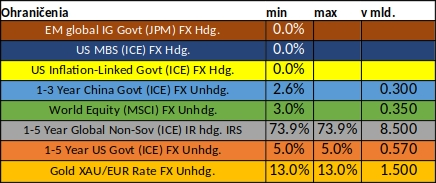
\includegraphics[width=1.1\textwidth]{Figures/constraints}
			\end{column}
			\pause\begin{column}{0.48\textwidth}
				\[
				\begin{aligned}
					&\min_{w_1, \ldots, w_n}ES_{5\%}^{5yr}(w_1, \ldots, w_n, \Omega) \\\pause
					s.t. &w_1 + \ldots + w_n = 1 \\\pause
					&\Omega = 11.52\\\pause
					&w_1 + w_2 + w_3 + w_4 + w_5 = \frac{0.65 + 0.3}{\Omega} \\\pause
					&w_4 > 0.026, \ w_5 > 0.03 \\\pause
					&w_6 = 0.739, \ w_7 = 0.05, \ w_8 = 0.13 \\\pause
					&ES_{1\%}^{1yr}(w_1, \ldots, w_n, \Omega) \leq 0.4
				\end{aligned}
				\]
			\end{column}
		\end{columns}
		
	\end{itemize}
\end{frame}

\begin{frame}{Príklad optimalizácie č. 2}
	\begin{itemize}
		\item Nech $w_1, \ldots, w_n$ sú váhy portfólia, $w_1 + w_2 + \ldots, w_n = 1$. Majme scenár č.2 kde investor prispôsobí veľkosť portfólia $\Omega$ optimálnym váham.
		\item Optimalizačný problém by vyzeral napríklad nasledovne:
		\begin{columns}
			\begin{column}{0.48\textwidth}
				\centering
				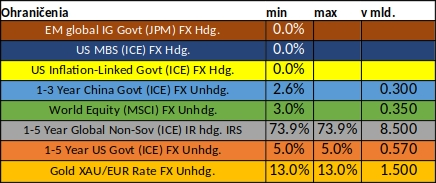
\includegraphics[width=1.1\textwidth]{Figures/constraints}
			\end{column}
			\begin{column}{0.48\textwidth}
				\[
				\begin{aligned}
				&\min_{w_1, \ldots, w_n, \Omega}ES_{5\%}^{5yr}(w_1, \ldots, w_n, \Omega) \\\pause
				s.t. &w_1 + \ldots + w_n = 1 \\\pause
				&w_4 > 0.026, \ w_5 > 0.03 \\\pause
				&w_6 = 0.739, \ w_7 = 0.05, \ w_8 = 0.13 \\\pause
				&w_8 = \frac{1.5}{\Omega}\\\pause
				&ES_{1\%}^{1yr}(w_1, \ldots, w_n, \Omega) \leq 0.4
				\end{aligned}
				\]
			\end{column}
		\end{columns}
	\end{itemize}
\end{frame}


\begin{frame}{Účelová funkcia vs. ohraničenia}
	\begin{itemize}
		\item Okrem rôznych prístupov k veľkosti portfólia je možné optimalizovať rôzne ciele za rôznych ohraničení.
		\item Možné ciele:		
		\begin{itemize}
			\item Mean - Variance optimalizácia
			\item Expected shortfall
			\begin{itemize}
				\item dá sa linearizovať, viď Rockafellar and Uryasev (2000)
				\item rôzne časové horizonty (1 rok, 5-7 rokov)
				\item rôzne pravdepodobnostné hladiny (95\%, 99\%)
			\end{itemize}
			\item minimalizovať $P($výnos $<X)$
		\end{itemize}
		\pause\item Možné ohraničenia:
		\begin{itemize}
			\item Expected shortfall < $X$ (opäť rôzne varianty)
			\item $P($výnos $<X) < Y$
			\item Minimálny očakávaný výnos.
			\item Maximálna akceptovaná variancia portfólia.
			\item Fixné zložky portfólia.
		\end{itemize}
	\end{itemize}
	\centering
	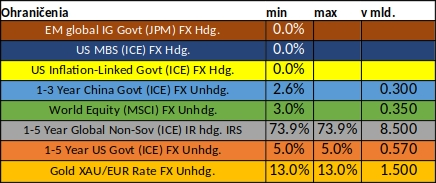
\includegraphics[width=0.6\textwidth]{Figures/constraints}
\end{frame}

\section{Výstup}
\begin{frame}{Výstup z projektu}
	\begin{itemize}
		\item Optimalizácia rôznych kombinácií ohraničení a cieľov, konsolidácia výsledkov do jedného datasetu, vytvorenie GUI pre používateľa v PowerBI / RShiny.
		\item Modulárny prístup k optimalizácii, používateľom zvoliteľné jednotlivé časti:
		\begin{itemize}
			\item Prístup k optimalizácii - scenár 1 vs. scenár 2.
			\item Cieľ optimalizácie - účelová funkcia (mean-var, ES, min $P($výnos $<X)$ ).
			\item Ohraničenia (ES, $P($výnos $<X) < Y$, min exp. výnos, max variance, ... ).
			\item [optional] Spôsob odhadu budúcich výnosov.
		\end{itemize}
		\pause\item Výstupom grafické zobrazenie:
		\begin{itemize}
			\item Hustota rozdelenia očakávanej hodnoty takéhoto portfólia vo viacerých časových horizontoch, napr. 1yr, 5yrs.
			\item Optimálne váhy porfólia.			
			\item Zaujímavé parametre pre všetky horizonty: VaR, Expected shortfall (CVar), expected return + variance, $P($výnos $<X) < 0$.
		\end{itemize}
	\end{itemize}	
\end{frame}

\begin{frame}{Cieľ + sumarizácia}
	\begin{itemize}
		\item Vytvoriť ucelený framework pre SAA, ktorý by okrem nájdenia optimálneho portfólia umožnil investorovi dynamicky meniť optimálne portfólio vzhľadom na zmenu v preferenciách.
		\pause\item Milestones:
		\begin{itemize}
			\item Model na predpovedanie budúcich výnosov, robustná parametrizácia pomocou Vine kopúl.
			\item Optimálne portfólio vzhľadom na expected shortfall, linearizácia, research možných ohraničení vzhľadom na numerickú náročnosť.
			\item Konsolidovaný výstup s dynamickým GUI pre investora na porovnanie očakávaných výnosov pre rôzne prístupy k optimalizácii.
		\end{itemize}
		\pause\item Pridaná hodnota:
		\begin{itemize}
			\item Odhad budúcich výnosov robustným modelom.
			\item Numericky priechodná optimalizácia expected shortfall.
			\item Ujasnenie predstavy o preferenciách investora / feedback mechanizmus.
		\end{itemize}
	\end{itemize}	
\end{frame}
\end{document}

